\documentclass[t,usepdftitle=false]{beamer}
\usepackage[utf8]{inputenc}
\usetheme{Warsaw}
\usepackage{xcolor}

\usepackage{etex}
\usepackage{pictex}
\usepackage{tikz}
\usetikzlibrary{shapes,arrows}
\usepackage{pgfplots}

\usepackage{amsmath}
\usepackage{amscd}
\usepackage{pstricks, pst-node}

\usepackage{times}

\usepackage{ulem}

\usepackage{amsmath, amsthm}
\usepackage{listings}

% \setbeamercovered{transparent}
%\usecolortheme{crane}
\title[IFT3245]{IFT 3245\\Simulation et modèles}
\author[Fabian Bastin]{Fabian Bastin\\DIRO\\Université de Montréal}
\date{Automne 2016}

\def\be{\boldsymbol{e}}
\def\bu{\boldsymbol{u}}
\def\bv{\boldsymbol{v}}
\def\bx{\boldsymbol{x}}
\def\bA{\boldsymbol{A}}
\def\cS{\mathcal{S}}

\def\rit{\mathcal{R}}

\begin{document}
\frame{\titlepage}

\begin{frame}
\frametitle{Générateur récursif multiple (MRG)}

Nous pouvons généraliser la récurrence du GCL par
\[
  {x_n} = (a_1 x_{n-1} + \cdots + a_k x_{n-k}) \mod {m}, \quad  
  {u_n} = x_n / m.
\]

\mbox{}

En pratique, on prendra plutôt $u_n = (x_n + 1) / (m+1)$,
ou encore $u_n = x_n/(m+1)$ si $x_n>0$ et $u_n = m/(m+1)$ sinon, mais
la structure demeure essentiellement la même.

\mbox{}

Si $k=1$, nous retrouvons le générateur à congruence linéaire
classique, avec $c = 0$.

\mbox{}

L'état à l'étape $n$ est
$s_n = {\bx_n} = (x_{n-k+1},\dots,x_n)^T$.\\
Espace d'états: $\mathcal{Z}_m^k$, de cardinalité $m^k$.\\
La période maximale est ${\rho} = m^k-1$, pour $m$ premier.

\end{frame}

\begin{frame}
\frametitle{Polynôme caractéristique}

On associe au MRG le polynôme caractéristique:
\[
  P(z) = z^k - a_1 z^{k-1} - \cdots - a_k
       = -\sum_{j=0}^k a_j z^{k-j},
\]
où $a_0=-1$.

\mbox{}

Pour $k > 1$, pour avoir une période maximale, il est possible de
montrer qu'il suffit d'avoir au moins deux coefficients non nuls, dont
$a_k$.
Ainsi, la récurrence la plus économique a la forme:
\[
 x_n = (a_r x_{n-r} + a_k x_{n-k}) \mod m,      \]
avec $0 < r < k$.

\end{frame}

\begin{frame}
\frametitle{$m=2^e$}

Une erreur fréquente, commise en particulier par les informaticiens
peu au fait des statistiques, est de considérer $m = 2^e$.

\mbox{}

Utiliser une puissance de 2 pour $m$ permet en effet de facilement calculer le
produit $ax \mod m$, et est parfois décrit comme efficace, ce qui est
vrai du point de la rapidité d'exécution.

\mbox{}

Les effets sur la période sont pourtant dommageables, vu que
\begin{itemize}
\item
pour $k=1$ et $e\ge 4$, on a $\rho \le 2^{e-2}$;
\item
pour $k > 1$, on a $\rho \le (2^k-1)2^{e-1}$.
\end{itemize}

\end{frame}

\begin{frame}
\frametitle{$m=2^e$: exemple}

Si $k=7$ et $m=2^{31}-1$, la période maximale est 
$(2^{31}-1)^7-1 \approx 2^{217}$.
Mais pour $m = 2^{31}$ on a $\rho \le (2^7-1)2^{31-1} < 2^{37}$, 
i.e. $2^{180}$ fois plus petit!

\mbox{}

Pire, si nous nous intéressons au $i^{\mbox{th}}$ bit le moins significatif,
pour $k=1$, la période de $x_n \mod 2^i$ ne peut pas dépasser
$\max (1, 2^{i-2})$.
Pour $k>1$, la période de $x_n \mod 2^i$ ne peut pas dépasser
$(2^k-1)2^{i-1}$.

\end{frame}

\begin{frame}
\frametitle{$m=2^e$: exemple}

Récurrence $x_n = 10205 x_{n-1} \mod 2^{15}$:
\begin {eqnarray*}
  x_0 ~=~ 12345 &=& 011000000111001_2 \\
  x_1 ~=~ 20533 &=& 101000000110101_2 \\
  x_2 ~=~ 20673 &=& 101000011000001_2 \\
  x_3 ~=~ ~7581 &=& 001110110011101_2 \\
  x_4 ~=~ 31625 &=& 111101110001001_2 \\
  x_5 ~=~ ~1093 &=& 000010001000101_2 \\
  x_6 ~=~ 12945 &=& 011001010010001_2 \\
  x_7 ~=~ 15917 &=& 011111000101101_2.\\
% x_8 ~=~ ~2009 &=& 000011111011001_2.\\
\end {eqnarray*}

\end{frame}

\begin{frame}[fragile]
\frametitle{$m=2^e$}

De tels générateurs restent populaires, mais sont à proscrire dans
des simulations dignes de ce nom.
Ainsi, la fonction \verb|ran48| reste présente dans les librairies C standards BSD.

\begin{small}
\begin {center}
\begin {tabular}{|l|r|r|l|}
\hline
 \phantom{12} $m$  & $a$ \phantom{12345}  & $c$\phantom{1234} & \phantom{12345} Source \\
\hline
 $2^{24}$    & 1140671485 & 12820163 & early MS VisualBasic \\
 $2^{31}$    &     65539  &    0  & RANDU (IBM) \\
 $2^{31}$    & 134775813  &    1  & early Turbo Pascal \\
 $2^{31}$    & 1103515245 & 12345 & {\tt rand()} in BSD ANSI C \\
 $2^{32}$    &     69069  &    1  & VAX/VMS systems \\ %(\cite{sKAR91a})\\
 $2^{32}$    & 2147001325 & 715136305  & BCLP language \\
 $2^{35}$    & $5^{15}$   & 7261067085 & Knuth (1998) \\
 $2^{48}$    & 68909602460261 &     0  & Fishman (1990) \\
 $2^{48}$    &    25214903917 &    11  & Unix's {\tt rand48()}  \\
 $2^{48}$    & 44485709377909 &     0  & CRAY system \\ %(\cite{rDEM90a})\\
 $2^{59}$    &  $13^{13}$     &     0  & NAG Fortran/C library  \\
\hline
\end {tabular}
\end {center}
\end{small}

\end{frame}

\begin{frame}
\frametitle{Générateurs à sous-suites multiples}

Afin de pouvoir adéquatement représenter les différentes variables aléatoires, il peut être intéressants de pouvoir instancier des générateurs de variables aléatoires à volonté, et faire évoluer ceux-ci en parallèle, plutôt que d'utiliser un seul générateur et transformer les tirs dans les distributions voulues à la volée.

\mbox{}

Nous voudrions pouvoir utiliser plusieurs fois un même générateur au sein d'un programme, mais en débutant avec des semences différentes afin de produire des suites aléatoires différentes.

\end{frame}

\begin{frame}
\frametitle{Générateurs à sous-suites multiples}

Une première approche consiste à créer plusieurs générateurs, en
spécifiant manuellement ces semences.
Le danger majeur de cette approche est qu'il est difficile de prévoir
la position des ces semences dans la séquence aléatoire, ce qui peut
conduire à produire des séquences fortement corrélées.
Le risque est d'autant plus élevé que la période du générateur est faible.

\end{frame}

\begin{frame} 
\frametitle{Exemple}

Soit $X$, $Y$, deux variables aléatoires normales $N(0,1)$ indépendantes.
Il est possible de montrer que le rapport $X/Y$ suit une distribution
de Cauchy.

\mbox{}

Générons ce rapport à l'aide du GCL Standard Minimal, avec 1 comme semence au
numérateur, et 2 au dénominateur.\\
\begin{center}
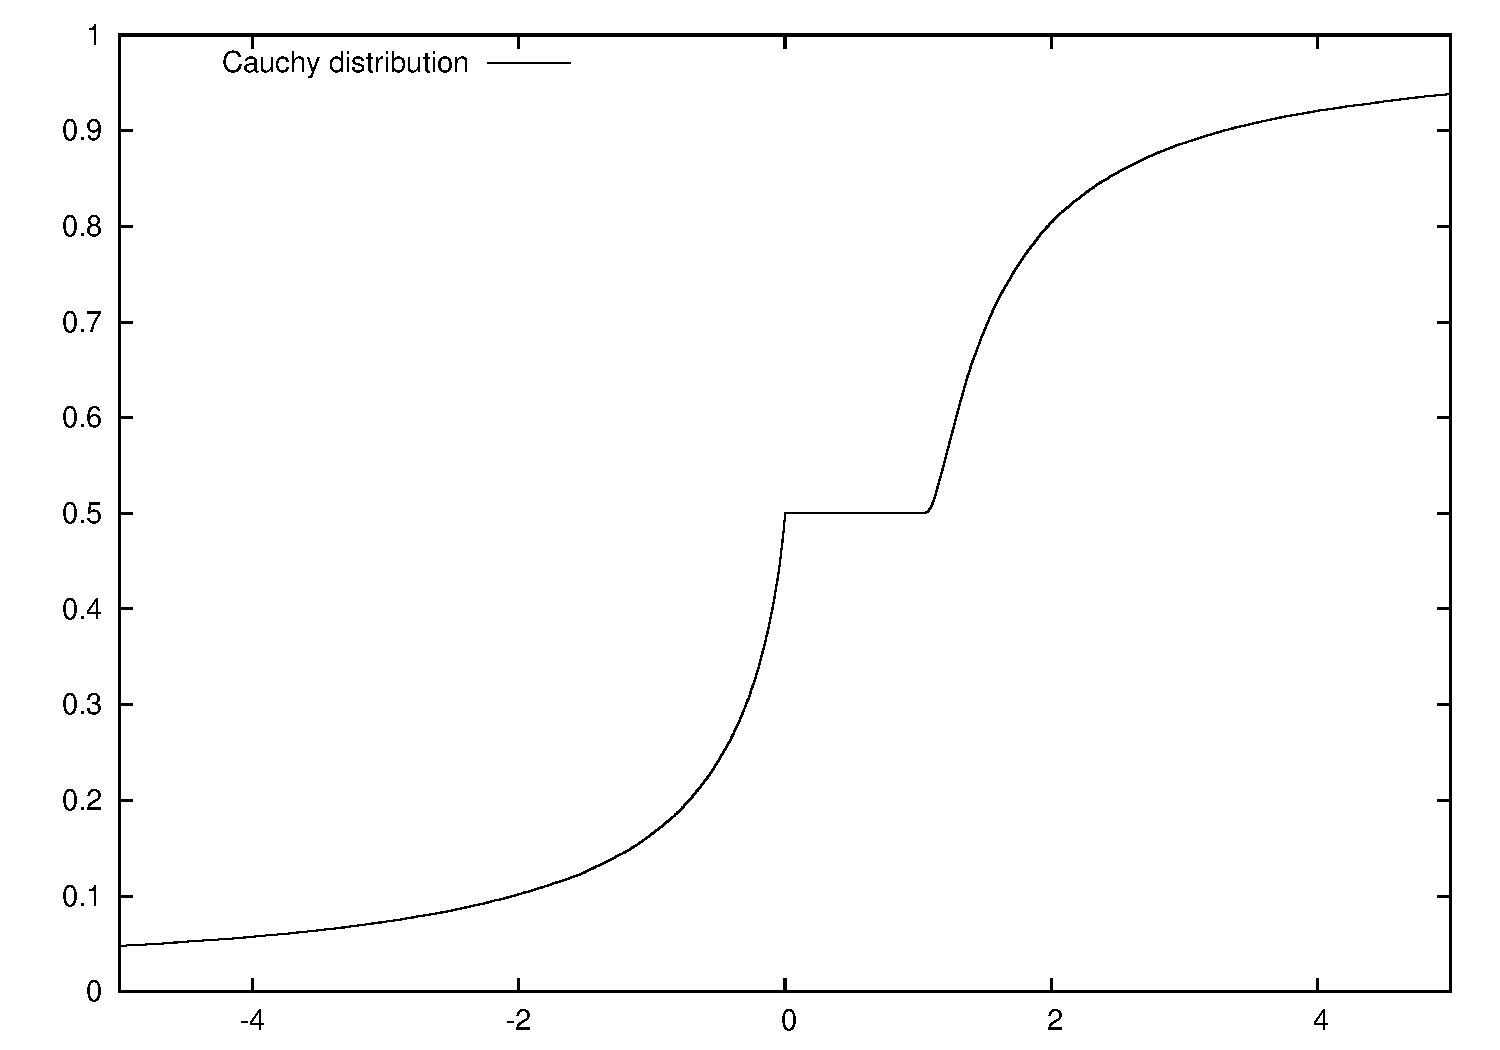
\includegraphics[width=0.5\linewidth]{cauchy_bad.pdf}
\end{center}

\end{frame}

\begin{frame}[fragile]
\frametitle{Générateurs à sous-suites multiples}

Il est ainsi utile de pouvoir partitionner ces suites (ou ``streams'') en sous-suites.

\begin{center}
%% see The TeXbook, Exercice 10.4
\def\tick#1#2{\vrule height 0pt depth #1pt width #2pt}
\def\enskip{\hskip.5em\relax}
\def\ld{\hbox to 0.24 in{\vtop{\kern1.5pt\hbox{\dotfill}}}}
\def\ts{\enskip\tick41}
\def\suba{\hbox to 1.0in {\vtop
 {\hbox to 1.0in{\hbox to .33in{\hrulefill}\hbox to .15in{\dotfill}\hrulefill}
  \hbox to 1.0in{{\tick{12}{2}}\ts\ts\ts\ts\ts\ts\ts\hfill\ts\enskip}}}}
\def\subb{\hbox to 1.0in {\vtop
 {\hbox to 1.0in{\hbox to .42in {\hrulefill}
         \hbox to .12in {\dotfill}\hbox to .06in {\hrulefill}}
  \hbox to 1.0in{{\tick{12}{2}}\ts\ts\ts\ts\ts\ts\ts\ts\hfill\ts\enskip}}}}

\setbox0=\vbox{\hsize=0.5in
\[
\hskip 0.3in
\vbox{\offinterlineskip
{\hskip 1.65in \hbox to 1.0in{\hfil\hskip1.07em 
   \emph{ }\hfil}\hfill}
\vskip 0pt
{\hskip 1.65in \hbox to 1.0in{\hfil\hskip1.07em 
   \emph{état}\hfil}\hfill}
\vskip 0pt
{\hskip 1.65in \hbox to 1.0in{\hfil\hskip1.0em 
   ${\Downarrow}$\hfil}
    \hfill}
\vtop {\offinterlineskip\hskip 0.0in \hbox to 7.5 true in
       {\suba\suba\subb\suba{\tick{12}{2}}
        \hbox to .12in {\hrulefill}\hbox to .24in{\dotfill}}}
        \vskip .1pt
{\hskip -0.5in\hbox to 0.75 in{\hfil début suite\hfil}\hbox to 1.65
  in{\hfil prochaine sous-suite\hfil}\hbox to 2.3
  in{\hfil prochaine suite\hfil}
\hfil}
\vskip .1pt }
\]
}
\box0
\end{center}

\end{frame}

\begin{frame}
\frametitle{Sauts entre suites}

Pour passer d'une suite à une autre, il est nécessaire de pouvoir
calculer un point de la récurrence sans devoir générer tous les points
intermédiaires.
Or, nous pouvons écrire
\[
  \bx_n = \bA \bx_{n-1} \mod m 
        = \begin{pmatrix}0 & 1 & \cdots & 0 \cr
                   \vdots &  & \ddots & \vdots \cr
                   0 & 0 & \cdots & 1 \cr
                   a_k & a_{k-1} & \cdots & a_1 \cr
   \end{pmatrix} \bx_{n-1} \mod m.
\]
Ainsi
\[
 \bx_{n+\nu} = \bA^\nu \bx_{n} \mod m 
    = (\bA^\nu \mod m) \bx_{n} \mod m.
\]

\end{frame}

\begin{frame}
\frametitle{Sauts entre suites}

Nous pouvons précalculer $\bA^\nu \mod m$ au moyen de la procédure suivante:
\begin{multline*}
  \bA^\nu \mod m = \\ \begin{cases}
    (\bA^{\nu/2} \mod m) (\bA^{\nu/2} \mod m) \mod m
                           & \mbox{ si $\nu$ est pair;} \\
    \bA (\bA^{\nu-1} \mod m) \mod m
                           & \mbox{ si $\nu$ est impair.}
 \end{cases}
\end{multline*}
%Avec la représentation polynômiale,
%\[
%  p_{n+\nu}(z) = z^\nu p_n(z) \mod P(z) 
%   = (z^\nu \mod P(z)) p_n(z) \mod P(z),
%\]
%oô $z^\nu \mod P(z)$ peut être précalculé.

\end{frame}

\end{document}
